%%%%%%%%%%%%%%%%%%%%%%%%%%%%%%%%%%%%%%%%%
% Jacobs Portrait Poster
% LaTeX Template
% Version 1.0 (31/08/2015)
% (Based on Version 1.0 (29/03/13) of the landscape template
%
% Created by:
% Computational Physics and Biophysics Group, Jacobs University
% https://teamwork.jacobs-university.de:8443/confluence/display/CoPandBiG/LaTeX+Poster
% 
% Further modified by:
% Nathaniel Johnston (nathaniel@njohnston.ca)
%
% Portrait version by:
% John Hammersley
%
% The landscape version of this template was downloaded from:
% http://www.LaTeXTemplates.com
%
% License:
% CC BY-NC-SA 3.0 (http://creativecommons.org/licenses/by-nc-sa/3.0/)
%
%%%%%%%%%%%%%%%%%%%%%%%%%%%%%%%%%%%%%%%%%

%----------------------------------------------------------------------------------------
%	PACKAGES AND OTHER DOCUMENT CONFIGURATIONS
%----------------------------------------------------------------------------------------

\documentclass[final]{beamer}

\usepackage[scale=1.24]{beamerposter} % Use the beamerposter package for laying out the poster

\usetheme{confposter} % Use the confposter theme supplied with this template

\setbeamercolor{block title}{fg=ngreen,bg=white} % Colors of the block titles
\setbeamercolor{block body}{fg=black,bg=white} % Colors of the body of blocks
\setbeamercolor{block alerted title}{fg=white,bg=dblue!70} % Colors of the highlighted block titles
\setbeamercolor{block alerted body}{fg=black,bg=dblue!10} % Colors of the body of highlighted blocks
% Many more colors are available for use in beamerthemeconfposter.sty

%-----------------------------------------------------------
% Define the column widths and overall poster size
% To set effective sepwid, onecolwid and twocolwid values, first choose how many columns you want and how much separation you want between columns
% In this template, the separation width chosen is 0.024 of the paper width and a 4-column layout
% onecolwid should therefore be (1-(# of columns+1)*sepwid)/# of columns e.g. (1-(4+1)*0.024)/4 = 0.22
% Set twocolwid to be (2*onecolwid)+sepwid = 0.464
% Set threecolwid to be (3*onecolwid)+2*sepwid = 0.708

\newlength{\sepwid}
\newlength{\onecolwid}
\newlength{\twocolwid}
\newlength{\threecolwid}
\setlength{\paperwidth}{36in} % A0 width: 46.8in
\setlength{\paperheight}{48in} % A0 height: 33.1in
\setlength{\sepwid}{0.024\paperwidth} % Separation width (white space) between columns
\setlength{\onecolwid}{0.22\paperwidth} % Width of one column
\setlength{\twocolwid}{0.464\paperwidth} % Width of two columns
\setlength{\threecolwid}{0.708\paperwidth} % Width of three columns
\setlength{\topmargin}{-0.5in} % Reduce the top margin size
%-----------------------------------------------------------

\usepackage{graphicx}  % Required for including images

\usepackage{booktabs} % Top and bottom rules for tables

\usepackage{url} % Top and bottom rules for tables
\usepackage{fontawesome}
% Decorate links:
\definecolor{linkcolor}{HTML}{003399}  % from https://gigaom.com/2009/07/09/when-it-comes-to-links-color-matters/
\newcommand{\colorify}[1]{\textcolor{linkcolor}{#1}}
\newcommand{\mylink}[1]{\href{#1}{\colorify{#1}}}
\newcommand{\mylinkn}[2]{\href{#1}{\colorify{#2}}}
\newcommand{\mylinkb}[2]{\href{#1}{#2}}
\newcommand{\mylinkm}[1]{\href{mailto:#1?subject=Your poster at 2017 NSLS-II and CFN Users' Meeting}{\colorify{#1}}}
\newcommand{\mylinkt}[1]{\href{tel:#1}{#1}}

%----------------------------------------------------------------------------------------
%	TITLE SECTION 
%----------------------------------------------------------------------------------------

\title{Sirepo --- software framework for X-ray sources and optics simulations} % Poster title

%\author{John Smith, James Smith and Jane Smith} % Author(s)

%\institute{Department and University Name} % Institution(s)

\author{Maksim S. Rakitin,\inst{a}* Paul Moeller,\inst{b, c} Rob Nagler,\inst{b} David L. Bruhwiler \inst{b} and Oleg Chubar\inst{a}}
\institute{\faInstitution{} \inst{a} NSLS-II, Brookhaven National Laboratory, Upton, NY~~~\faInstitution{} \inst{b} RadiaSoft LLC, Boulder, CO~~~\faInstitution{} \inst{c} Bivio LLC, Boulder, CO}

%----------------------------------------------------------------------------------------

\begin{document}

\addtobeamertemplate{headline}{} 
{
\begin{tikzpicture}[remember picture,overlay] 
\node [shift={(+3.8cm, -3.5cm)}] at (current page.north west){\includegraphics[height=5cm]{images/Sirepo_logo_symbol.png}}; 
\end{tikzpicture} 
}

\addtobeamertemplate{headline}{} 
{
\begin{tikzpicture}[remember picture,overlay] 
\node [shift={(7.0cm, +2.5cm)}] at (current page.south west){
\includegraphics[height=4.0cm]{images/bnl_logo.png}}; 
\end{tikzpicture} 

\begin{tikzpicture}[remember picture,overlay] 
\node [shift={(-8cm, +2.0cm)}] at (current page.south east){
\includegraphics[height=2.5cm]{images/radiasoft_logo.png}}; 
\end{tikzpicture} 
}

\addtobeamertemplate{block end}{}{\vspace*{2ex}} % White space under blocks
\addtobeamertemplate{block alerted end}{}{\vspace*{2ex}} % White space under highlighted (alert) blocks

\setlength{\belowcaptionskip}{2ex} % White space under figures
\setlength\belowdisplayshortskip{2ex} % White space under equations

\begin{frame}[t] % The whole poster is enclosed in one beamer frame

\begin{columns}[t] % The whole poster consists of three major columns, the second of which is split into two columns twice - the [t] option aligns each column's content to the top

\begin{column}{\sepwid}\end{column} % Empty spacer column

\begin{column}{\onecolwid} % The first column

%----------------------------------------------------------------------------------------
%	OBJECTIVES
%----------------------------------------------------------------------------------------

\begin{alertblock}{Objectives}

Sirepo allows to perform scientific simulations in a cloud:
\begin{itemize}
  \item Convenient and installation-free access to physical optics and accelerator codes (SRW, Elegant, WARP, \textit{etc.})
  \item Simulation of X-ray sources (undulators, damping wigglers, \textit{etc.})
  \item Simulation of wavefront propagation through optical system of X-ray beamlines
  \item Sharing the simulations with colleagues and collaborators
\end{itemize}

\end{alertblock}


%----------------------------------------------------------------------------------------
%	INTRODUCTION
%----------------------------------------------------------------------------------------

\begin{block}{\faInfoCircle{} Introduction}

\textbf{Sirepo} --- a browser-based GUI and framework for X-ray optics simulations, built on top of Synchrotron Radiation Workshop (SRW).

\vspace{1cm}

\textbf{SRW} --- a physical optics computer code, allowing simulation of entire experimental beamlines using the concept of a ``Virtual Beamline'' with the accurate treatment of the synchrotron radiation propagation through the X-ray optical system~\cite{Chubar1998_SRW, Chubar2002_SRW, Chubar2013_SRW}.
\end{block}

\begin{block}{\faLink{} Links}

\textbf{\faGears{} Use:}

\begin{itemize}
  \item[\faGear{}]~\mylinkn{https://beta.sirepo.com/light}{beta.sirepo.com/light} (publicly available)
  \item[\faGear{}]~\mylinkn{https://expdev.nsls2.bnl.gov/light}{expdev.nsls2.bnl.gov/light} (behind NSLS-II firewall)
  \item[\faGear{}]~\mylinkn{http://nsls2expdev1.bnl.gov:8000/light}{nsls2expdev1.bnl.gov:8000/light} (behind NSLS-II firewall)
\end{itemize}

\textbf{\faDownload{} Download (open source):}

\begin{itemize}
  \item[\faGithub{}]~\mylinkn{https://github.com/radiasoft/sirepo}{github.com/radiasoft/sirepo}
  \item[\faGithub{}]~\mylinkn{https://github.com/ochubar/SRW}{github.com/ochubar/SRW}
  \item[\faShip{}]~\mylinkn{https://hub.docker.com/r/radiasoft/sirepo/tags/}{hub.docker.com/r/radiasoft}
  \item[\faCloudDownload{}]~\mylinkn{https://atlas.hashicorp.com/radiasoft/boxes/sirepo}{atlas.hashicorp.com/radiasoft}
\end{itemize}

\end{block}

\begin{block}{\faUsers{} Users}
\begin{itemize}
  \item NSLS-II, LCLS, APS, ALS in the US
  \item ELETTRA in Italy
  \item European XFEL in Germany
  \item ESRF and SOLEIL in France
  \item PSI in Switzerland
  \item Diamond Light Source in UK
  \item LNLS in Brazil
\end{itemize}
\end{block}

%----------------------------------------------------------------------------------------

\end{column} % End of the first column

\begin{column}{\sepwid}\end{column} % Empty spacer column

\begin{column}{\twocolwid} % Begin a column which is two columns wide (column 2)

\begin{columns}[t,totalwidth=\twocolwid] % Split up the two columns wide column

\begin{column}{\onecolwid}\vspace{-.6in} % The first column within column 2 (column 2.1)

%----------------------------------------------------------------------------------------
%	MATERIALS
%----------------------------------------------------------------------------------------

\begin{block}{\faServer{} Server technologies}

\begin{itemize}
  \item \textbf{Python} --- widely used high-level programming language for general-purpose programming
  \item \textbf{Flask} --- lightweight framework for web development with Python based on Werkzeug WSGI toolkit
  \item \textbf{Nginx} --- industry standard HTTP server and a reverse proxy
  \item \textbf{JSON (JavaScript Object Notation)} --- a lightweight data-interchange format
  \item \textbf{Celery and RabbitMQ} --- asynchronous job queue and cluster management
  \item \textbf{Open MPI/mpi4py} --- technology used to run scientific codes in parallel across a cluster of computational nodes on a network
\end{itemize}

\end{block}

%----------------------------------------------------------------------------------------

\end{column} % End of column 2.1
%
\begin{column}{\onecolwid}\vspace{-.6in} % The second column within column 2 (column 2.2)

%----------------------------------------------------------------------------------------
%	METHODS
%----------------------------------------------------------------------------------------

\begin{block}{\faFirefox{} \faChrome{} \faInternetExplorer{} Client}

\begin{itemize}
  \item \faHtml5{} \textbf{HTML5} --- markup language used for structuring and presenting web content
  \item \faCss3{} \textbf{CSS3} --- style sheet language used for describing the presentation of a document written in a markup language
  \item \textbf{Bootstrap} --- HTML, CSS and JavaScript framework for developing cross-platform web
applications
  \item \textbf{AngularJS} --- structural framework for dynamic web apps
  \item \textbf{D3.js} --- JavaScript graphics library which is used to generate interactive plots in the browser. D3 supports large datasets and dynamic behaviors for interaction and animation.
\end{itemize}

\end{block}

%----------------------------------------------------------------------------------------

\end{column} % End of column 2.2
%
\end{columns} % End of the split of column 2 - any content after this will now take up 2 columns width

%----------------------------------------------------------------------------------------
%	IMPORTANT RESULT
%----------------------------------------------------------------------------------------

\begin{block}{\faLightbulbO{} Source page}

\begin{figure}
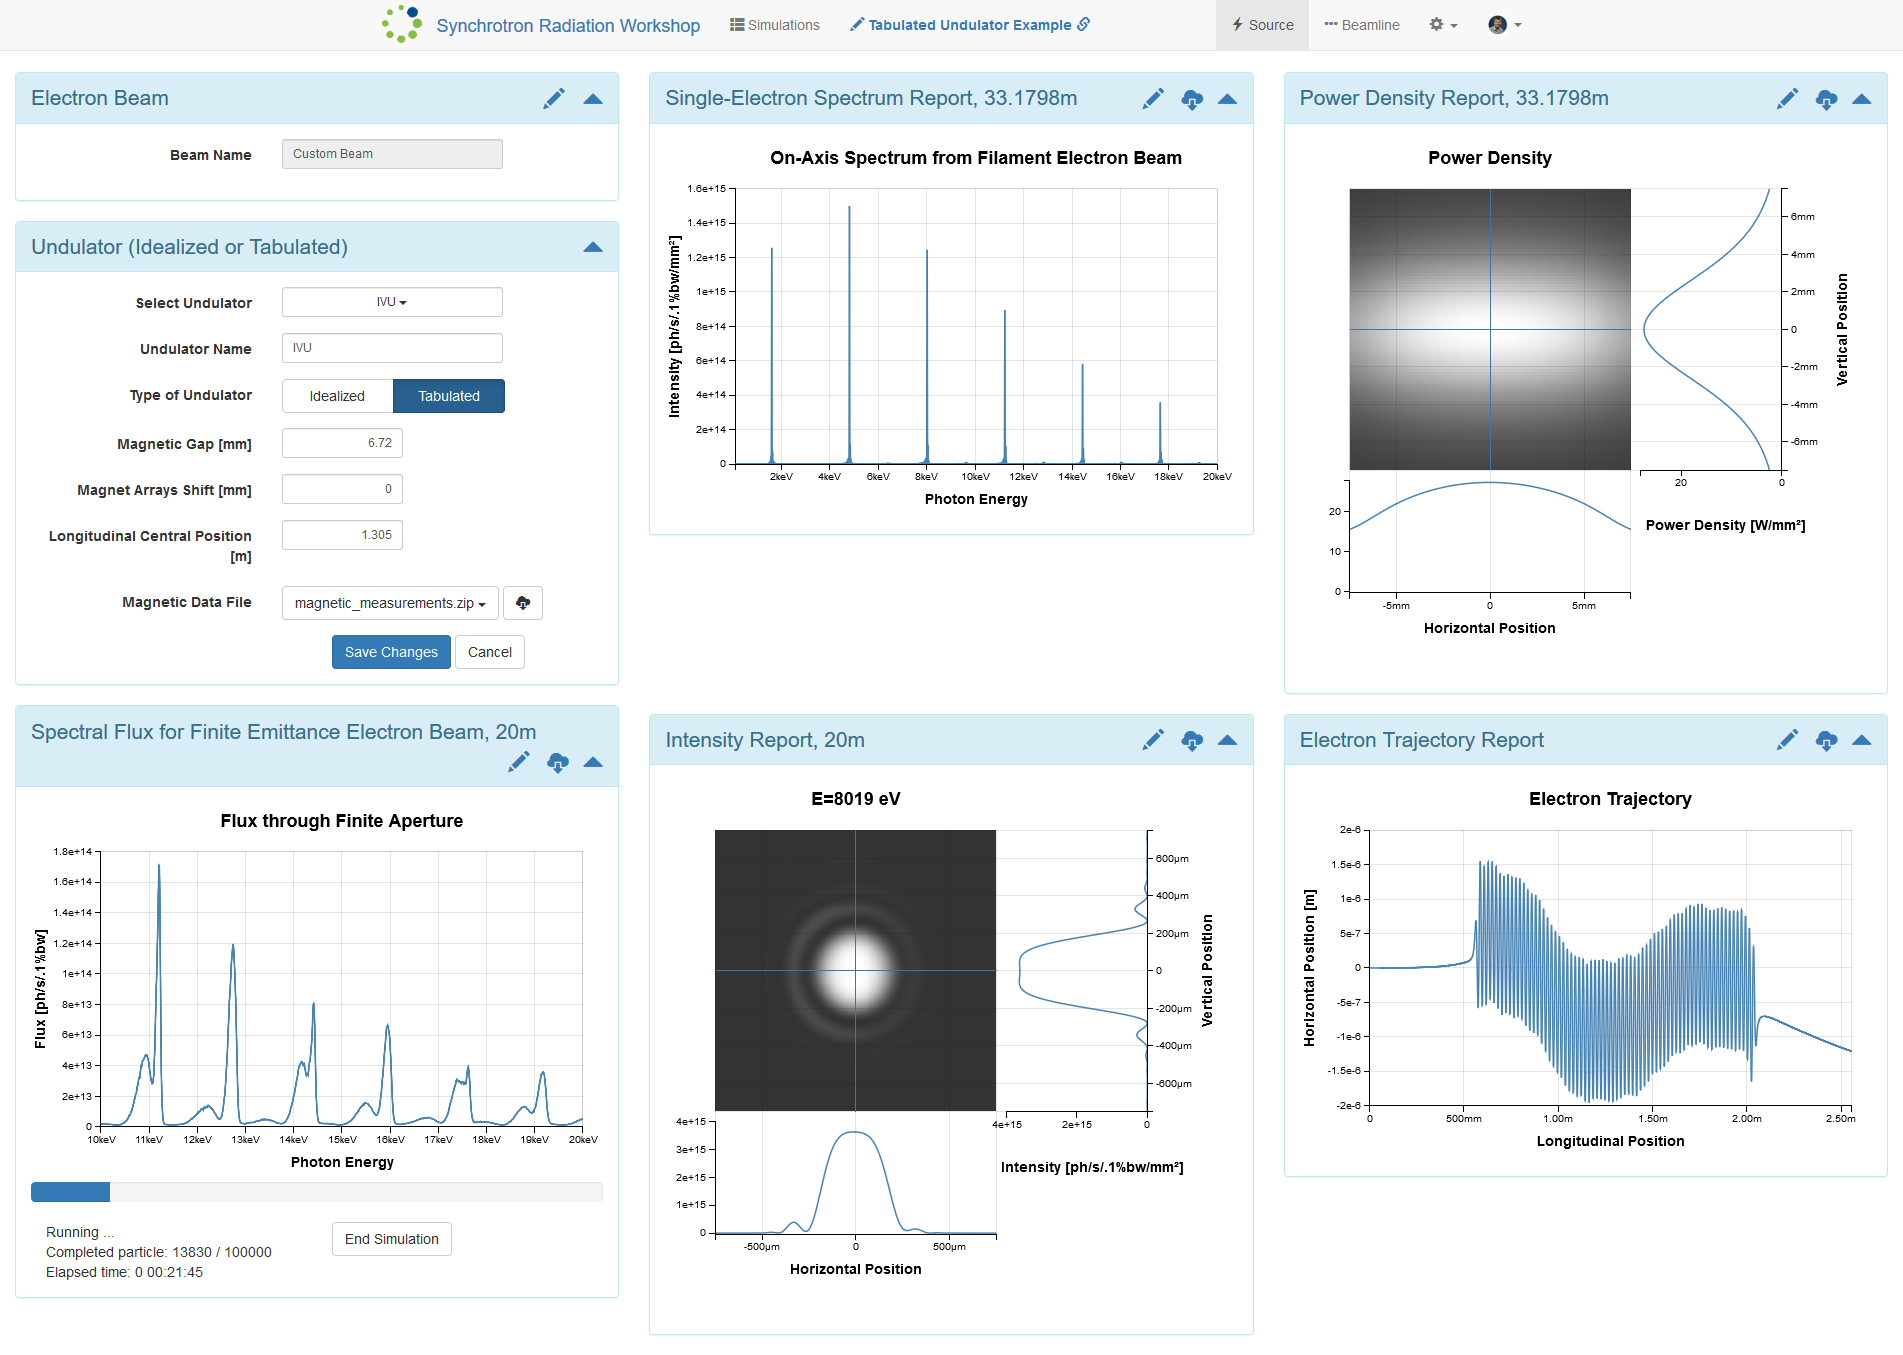
\includegraphics[width=0.85\linewidth]{images/source_page.png}
% \caption{Figure caption}
\end{figure}

\end{block} 


\begin{block}{\faSignOut{} \faEllipsisH{} \faBullseye{} Beamline page}

\begin{figure}
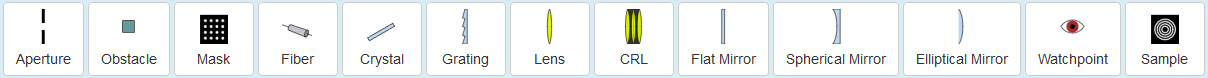
\includegraphics[width=0.85\linewidth]{images/toolbar_menu.png}
% \caption{Figure caption}
\end{figure}

\begin{figure}
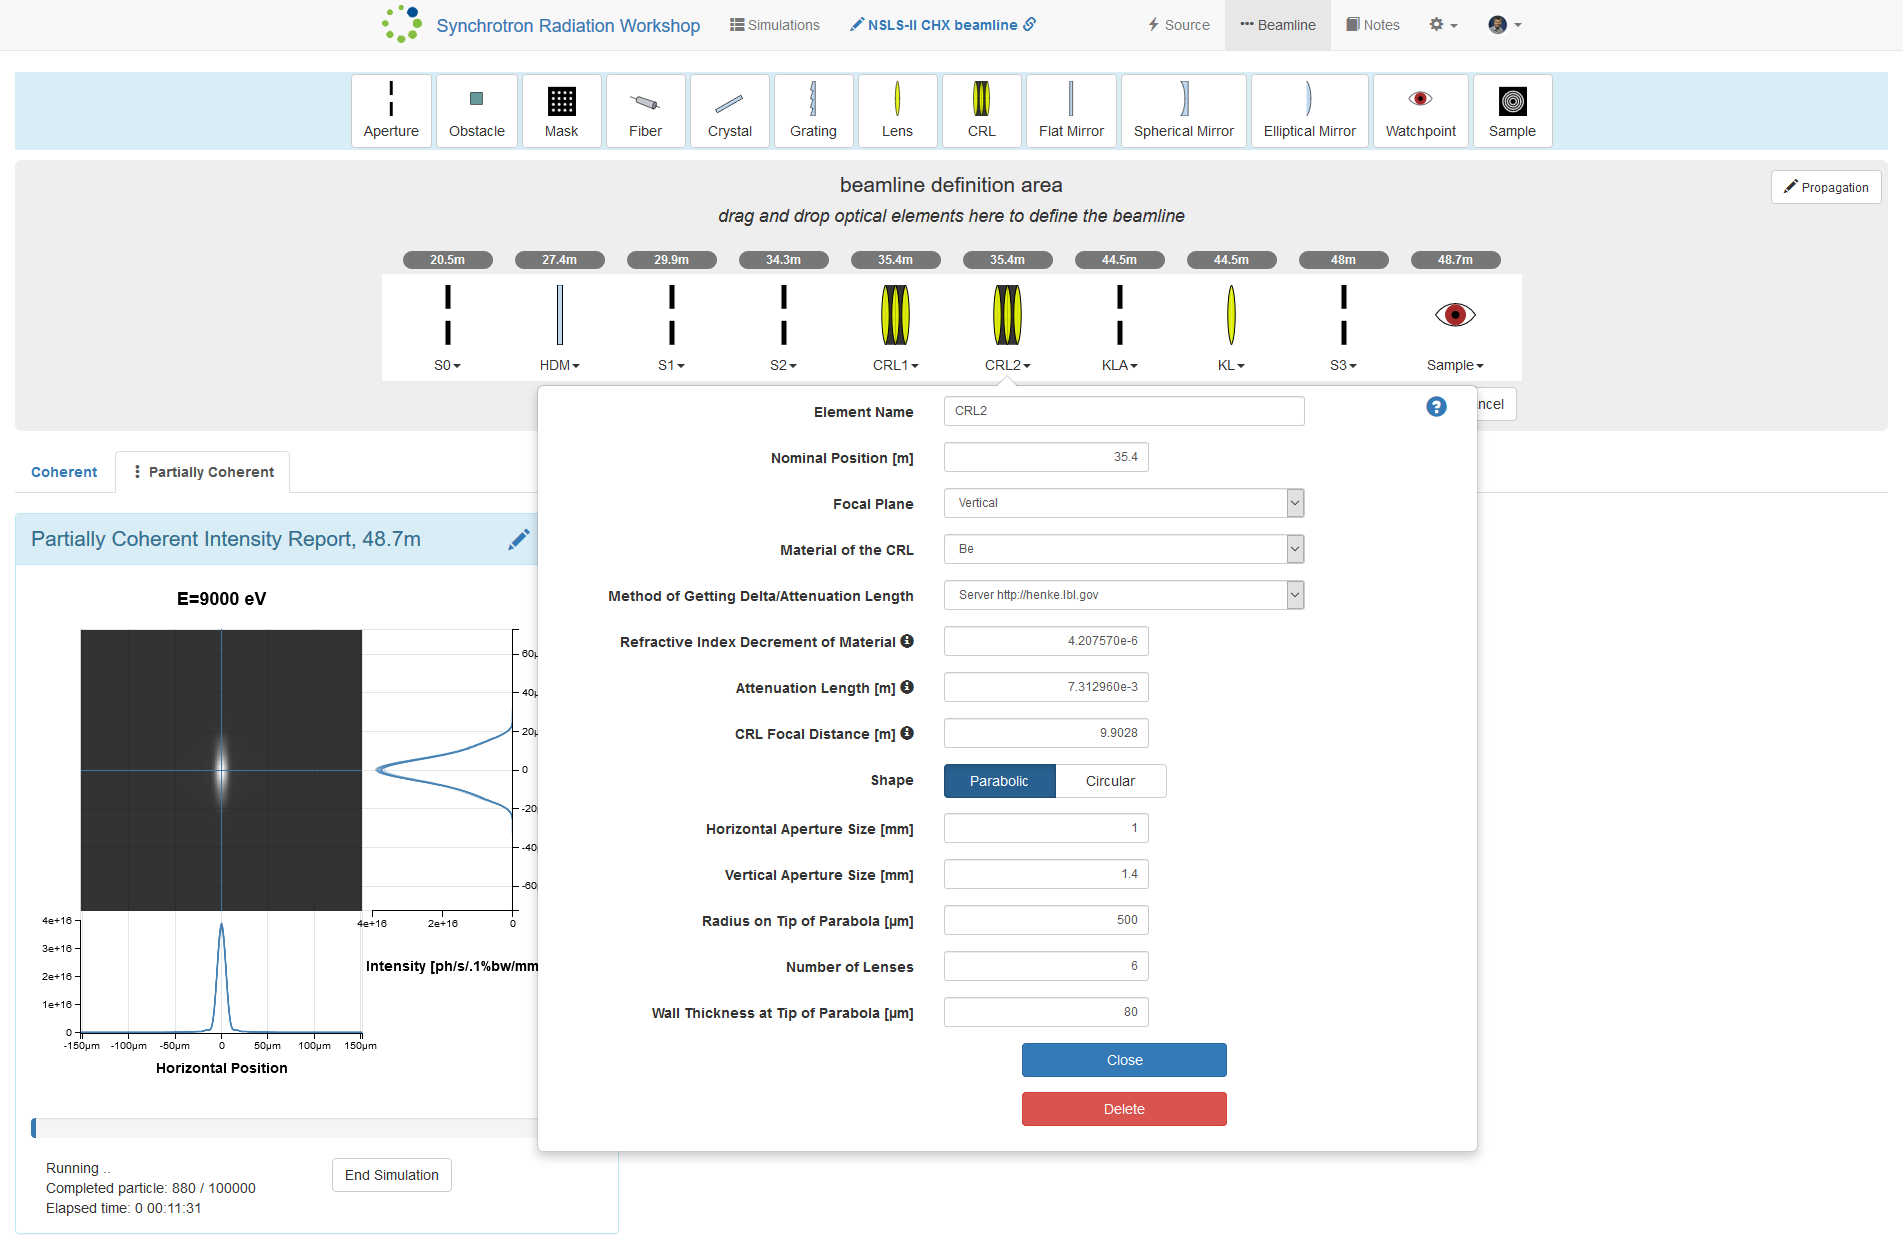
\includegraphics[width=0.85\linewidth]{images/beamline_page.png}
% \caption{Figure caption}
\end{figure}

\end{block}


%----------------------------------------------------------------------------------------

\end{column} % End of the second column

\begin{column}{\sepwid}\end{column} % Empty spacer column

\begin{column}{\onecolwid} % The third column

%----------------------------------------------------------------------------------------
%	CONCLUSION
%----------------------------------------------------------------------------------------

\begin{block}{\faFlag{} Conclusion}

\textbf{Sirepo} --- a browser-based open-source framework for X-ray optics simulations. Sirepo is interfaced with a number of leading codes in the fields of X-ray source and optics simulations (SRW and Shadow3) and particle accelerators (Elegant, Hellweg and Warp). Sirepo for SRW contains predefined textbook examples as well as simulations of the wavefront propagation through the real beamlines at NSLS-II. On the Source page users can optimize the source of the synchrotron radiation. On the Beamline page one can construct a ``virtual'' beamline emulating layout of a real experimental beamline. Sirepo is empowered with the interactive widgets and dynamically accessed data from the community databases for X-ray optics~\cite{stepanov, henke}. Simulation of experimental samples is implemented in Sirepo \& SRW.

\end{block}

%----------------------------------------------------------------------------------------
%	REFERENCES
%----------------------------------------------------------------------------------------

\begin{block}{\faBook{} References}

\nocite{*} % Insert publications even if they are not cited in the poster
\small{\bibliographystyle{unsrt}
\bibliography{sirepo} \vspace{-0.48cm}}

\end{block}

%----------------------------------------------------------------------------------------
%	ACKNOWLEDGEMENTS
%----------------------------------------------------------------------------------------

%\setbeamercolor{block title}{fg=red,bg=white} % Change the block title color

\begin{block}{\faThumbsOUp{} Acknowledgements}

\small{\rmfamily{The authors are thankful for the financial support of this work by the US DOE Office of Science, Office of Basic Energy Sciences under SBIR awards DE-SC0006284 and DE-SC0011237.}} \\

\end{block}

%----------------------------------------------------------------------------------------
%	CONTACT INFORMATION
%----------------------------------------------------------------------------------------

\setbeamercolor{block alerted title}{fg=black,bg=norange} % Change the alert block title colors
\setbeamercolor{block alerted body}{fg=black,bg=white} % Change the alert block body colors

\begin{alertblock}{\faSendO{} Contact Information}

~~~\faEnvelopeO~~\mylinkm{mrakitin@bnl.gov} \\
~~~\faGlobe~~\mylinkn{https://mrakitin.xyz}{mrakitin.xyz} \\
~~~\faGithub~~\mylinkn{https://github.com/mrakitin}{github.com/mrakitin} \\
~~~\faLinkedinSquare~~\mylinkn{https://www.linkedin.com/in/mrakitin}{linkedin.com/in/mrakitin} \\
~~~\faTwitter~~\mylinkn{https://twitter.com/mrakiti}{twitter.com/mrakiti} \\
~~~\faPhone~~\mylinkt{+1~(631)~344--8299} \\

\end{alertblock}

%----------------------------------------------------------------------------------------

\begin{minipage}[t]{0.48\linewidth}

\includegraphics[height=4.0cm]{images/qr_code_beta.jpg}

\includegraphics[height=4.0cm]{images/qr_code_github_radiasoft_sirepo.jpg}
\end{minipage}


\end{column} % End of the third column

\end{columns} % End of all the columns in the poster

\end{frame} % End of the enclosing frame

\end{document}
